%
% This is the LaTeX template file for lecture notes for EE 382C/EE 361C.
%
% To familiarize yourself with this template, the body contains
% some examples of its use.  Look them over.  Then you can
% run LaTeX on this file.  After you have LaTeXed this file then
% you can look over the result either by printing it out with
% dvips or using xdvi.
%
% This template is based on the template for Prof. Sinclair's CS 270.

\documentclass[twoside]{article}
\usepackage{graphicx}
\usepackage{amsmath}
\setlength{\oddsidemargin}{0.25 in}
\setlength{\evensidemargin}{-0.25 in}
\setlength{\topmargin}{-0.6 in}
\setlength{\textwidth}{6.5 in}
\setlength{\textheight}{8.5 in}
\setlength{\headsep}{0.75 in}
\setlength{\parindent}{0 in}
\setlength{\parskip}{0.1 in}

%
% The following commands set up the lecnum (lecture number)
% counter and make various numbering schemes work relative
% to the lecture number.
%
\newcounter{lecnum}
\renewcommand{\thepage}{\thelecnum-\arabic{page}}
\renewcommand{\thesection}{\thelecnum.\arabic{section}}
\renewcommand{\theequation}{\thelecnum.\arabic{equation}}
\renewcommand{\thefigure}{\thelecnum.\arabic{figure}}
\renewcommand{\thetable}{\thelecnum.\arabic{table}}

%
% The following macro is used to generate the header.
%
\newcommand{\lecture}[4]{
   \pagestyle{myheadings}
   \thispagestyle{plain}
   \newpage
   \setcounter{lecnum}{#1}
   \setcounter{page}{1}
   \noindent
   \begin{center}
   \framebox{
      \vbox{\vspace{2mm}
    \hbox to 6.28in { {\bf EE 382V: Social Computing
                        \hfill Fall 2018} }
       \vspace{4mm}
       \hbox to 6.28in { {\Large \hfill Lecture #1: #2  \hfill} }
       \vspace{2mm}
       \hbox to 6.28in { {\it Lecturer: #3 \hfill Scribe: #4} }
      \vspace{2mm}}
   }
   \end{center}
   \markboth{Lecture #1: #2}{Lecture #1: #2}
   %{\bf Disclaimer}: {\it These notes have not been subjected to the
   %usual scrutiny reserved for formal publications.  They may be distributed
   %outside this class only with the permission of the Instructor.}
   \vspace*{4mm}
}

%
% Convention for citations is authors' initials followed by the year.
% For example, to cite a paper by Leighton and Maggs you would type
% \cite{LM89}, and to cite a paper by Strassen you would type \cite{S69}.
% (To avoid bibliography problems, for now we redefine the \cite command.)
% Also commands that create a suitable format for the reference list.
\renewcommand{\cite}[1]{[#1]}
\def\beginrefs{\begin{list}%
        {[\arabic{equation}]}{\usecounter{equation}
         \setlength{\leftmargin}{2.0truecm}\setlength{\labelsep}{0.4truecm}%
         \setlength{\labelwidth}{1.6truecm}}}
\def\endrefs{\end{list}}
\def\bibentry#1{\item[\hbox{[#1]}]}

%Use this command for a figure; it puts a figure in wherever you want it.
%usage: \fig{NUMBER}{SPACE-IN-INCHES}{CAPTION}
\newcommand{\fig}[3]{
			\vspace{#2}
			\begin{center}
			Figure \thelecnum.#1:~#3
			\end{center}
	}
% Use these for theorems, lemmas, proofs, etc.
\newtheorem{theorem}{Theorem}[lecnum]
\newtheorem{lemma}[theorem]{Lemma}
\newtheorem{proposition}[theorem]{Proposition}
\newtheorem{claim}[theorem]{Claim}
\newtheorem{corollary}[theorem]{Corollary}
\newtheorem{definition}[theorem]{Definition}
\newenvironment{proof}{{\bf Proof:}}{\hfill\rule{2mm}{2mm}}

% **** IF YOU WANT TO DEFINE ADDITIONAL MACROS FOR YOURSELF, PUT THEM HERE:

\begin{document}
%FILL IN THE RIGHT INFO.
%\lecture{**LECTURE-NUMBER**}{**DATE**}{**LECTURER**}{**SCRIBE**}
\lecture{2}{August 25}{Vijay Garg}{Javier Palomares}
%\footnotetext{These notes are partially based on those of Nigel Mansell.}

% **** YOUR NOTES GO HERE:

% Some general latex examples and examples making use of the
% macros follow.  
%**** IN GENERAL, BE BRIEF. LONG SCRIBE NOTES, NO MATTER HOW WELL WRITTEN,
%**** ARE NEVER READ BY ANYBODY.
% * <javier.palomares.90@gmail.com> 2018-08-27T01:16:28.698Z:
%
% ^.
\section{Linear Programming}
Linear Programming involves finding the maximum possible value of some objective subject to some constraints. For example, we might want to maximize the harvest value of some plot of land where we can plant different crops. In linear programming models these type of problems are modeled as a set of  decision variables 
\newline \{$x_1,x_2,\ldots,x_n$\}
\newline and an objective function 
\newline $c_1 x_1 + c_2 x_2 +\ldots+ c_n x_n$ 
\newline subject to some constraints 
\newline $a_{11} x_1 + a_{12} x_2 + \ldots + a_{1n}x_n \leq b_1$ 
\newline $a_{21} x_1 + a_{22} x_2 + \ldots + a_{2n}x_n \leq b_2$ 
\newline $\vdots$
\newline $a_{m1} x_1 + a_{m2} x_2 + \ldots + a_{mn}x_n \leq b_m$ 
\newline $x_1,x_2, \ldots, x_n \geq 0$
\newline Linear programming only deals with problems that are linear with respect to the decision variables in the objective function and constraints.

\subsection{Example of Linear Programming}
Maximize the objective function \newline  $x_1 + x_2$ \newline subject to \newline
$2 x_1 + x_2 \leq 1 \newline x_1 + 2 x_2 \leq 1 \newline x_1,x_2 \geq 0 $

To solve the problem we need to find the point that maximizes the objective function within the union of the spaces defined by each of the constraints. This point is called the optimal solution, and the value the objective function takes at this space is called the optimal value. The space defined by the set of constraints is called the feasible space.

\begin{figure}[!ht]
  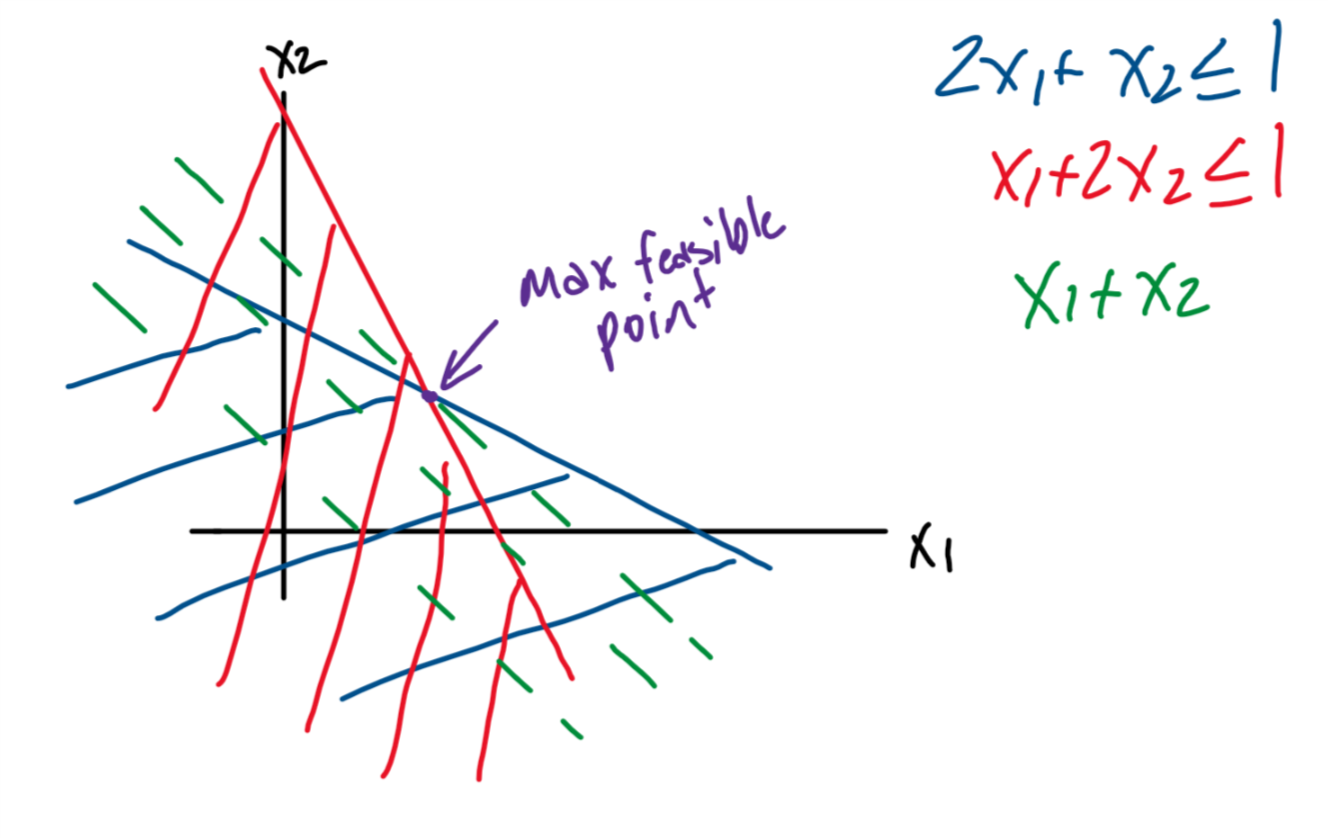
\includegraphics[width=3in]{LP_example.png}
  \caption{Finding optimal solution in the feasible space}
  \label{fig:lp_example}
\end{figure}

Figure \ref{fig:lp_example} shows the feasible space defined by the constraints. Possible values of the objective function correspond to the level sets of $x_1 + x_2$. Since the objective function grows as $x_1$ and $x_2$ grow, level sets up and to the right corresponding to a bigger value in the objective function. It turns out that the corner of the feasible space at $(x_1,x_2) = (1/3,1/3)$ is the optimal point. 

\subsection{Solution at corner points}
A lot of Linear Programming was formulated by George Dantzig who found that optimal points are always at the corners of the feasible space. He formulated this into the Simplex algorithm.

\section{Duality}
It turns out that every linear problem has an associated problem called the simplex. If the linear problem (called the primal) is a maximization problem, the dual is a minimization problem, and solutions to the dual problem are an upper limit on the optimal value to the primal problem. If the primal is a minimization problem, then the dual is a maximization problem.
Moreover, duality also states that the optimal value of the dual problem equals the optimal value of the primal.

\begin{figure}[!ht]
  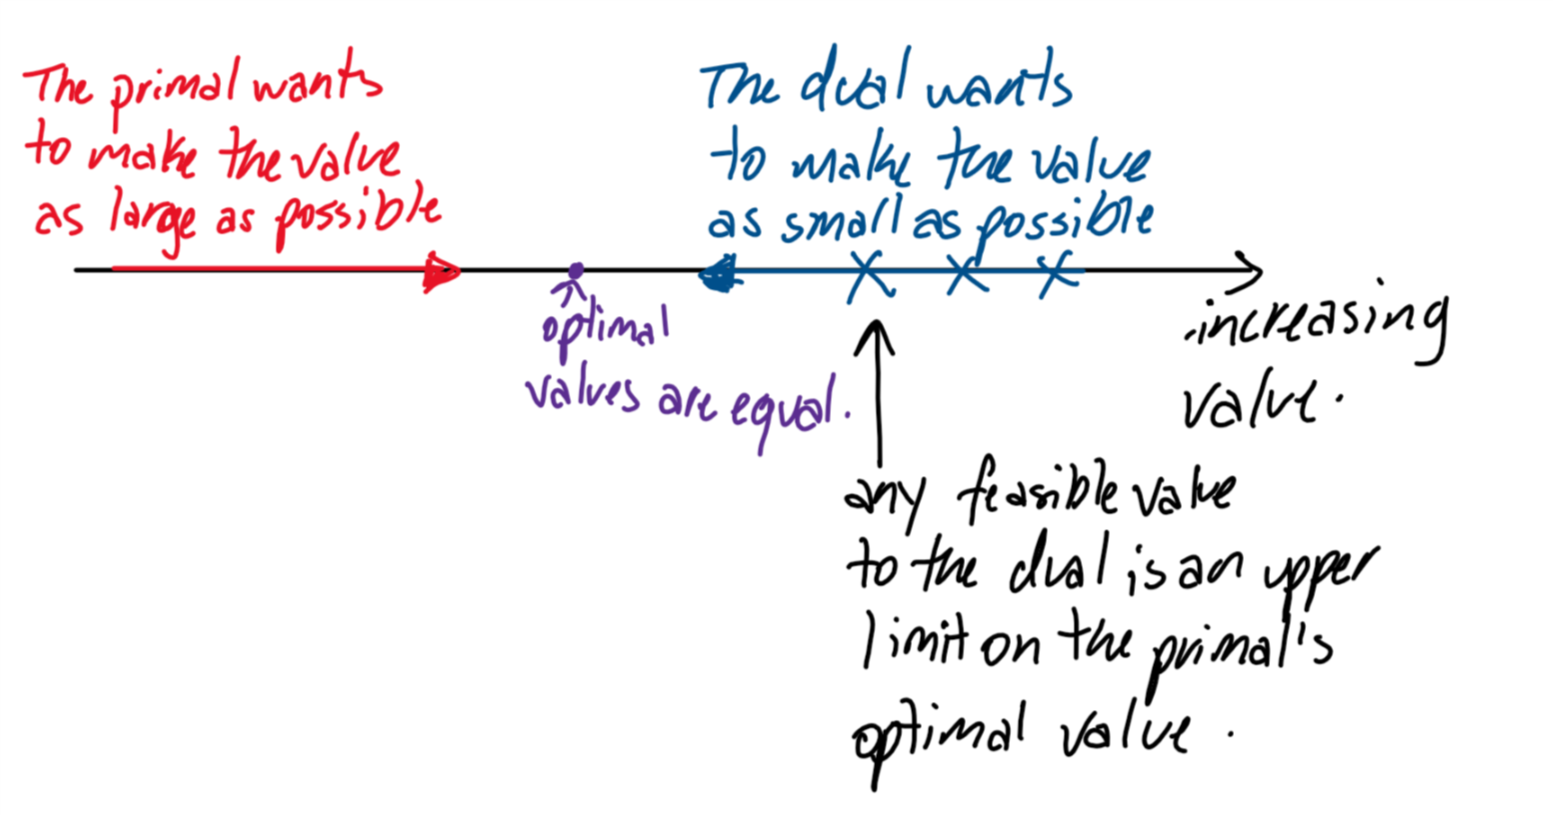
\includegraphics[width=3in]{dual_line.png}
  \caption{The dual places an upper limit on the primal's optimal value}
  \label{fig:dual_number_line}
\end{figure}

\subsection{Duality in practice}
If we can find a vertex cover for a bipartite graph of size n, then by duality, we can prove that there then there cannot exist a matching of size bigger than n. The minimization problem (finding a vertex cover) places an upper bound on the maximization problem (cardinality of the matching).

\subsection{Duality example}

minimize \newline 
$7x_1 + x_2 + 5x_3 $ \newline
subject to \newline
$x_1 - x_2 + 3 x_3 \geq 10 \newline
5 x_1 + 2x_2 -x_3 \geq 6 \newline
x_1,x_2,x_3 \geq 0 $


The dual problem is
\newline
\newline maximize 
\newline $ 10 p_1 + 6 p_2 $
\newline subject to
\newline $p_1 + 5 p_2 \leq 7$
\newline $-p_1 + 2 p_2 \leq 1 $
\newline $ 3 p_1 - p_2 \leq 5 $
\newline $p_1,p_2,p_3 \geq 0$

Duality tells us that if we find $any$ solution to the dual problem, even if it's not the optimal solution, with a value $V$, then the optimal value of the primal cannot be less than $V$.


\subsection{Max-Flow/Min-Cut}
In a max flow, the goal is to maximize the flow from a source node to a destination node subject to the constrained capacity of edges between intermediate nodes. Additionally, flow must be conserved, so the flow into an intermediate node is constrained to equal the flow out of a node.

\begin{figure}[!ht]
  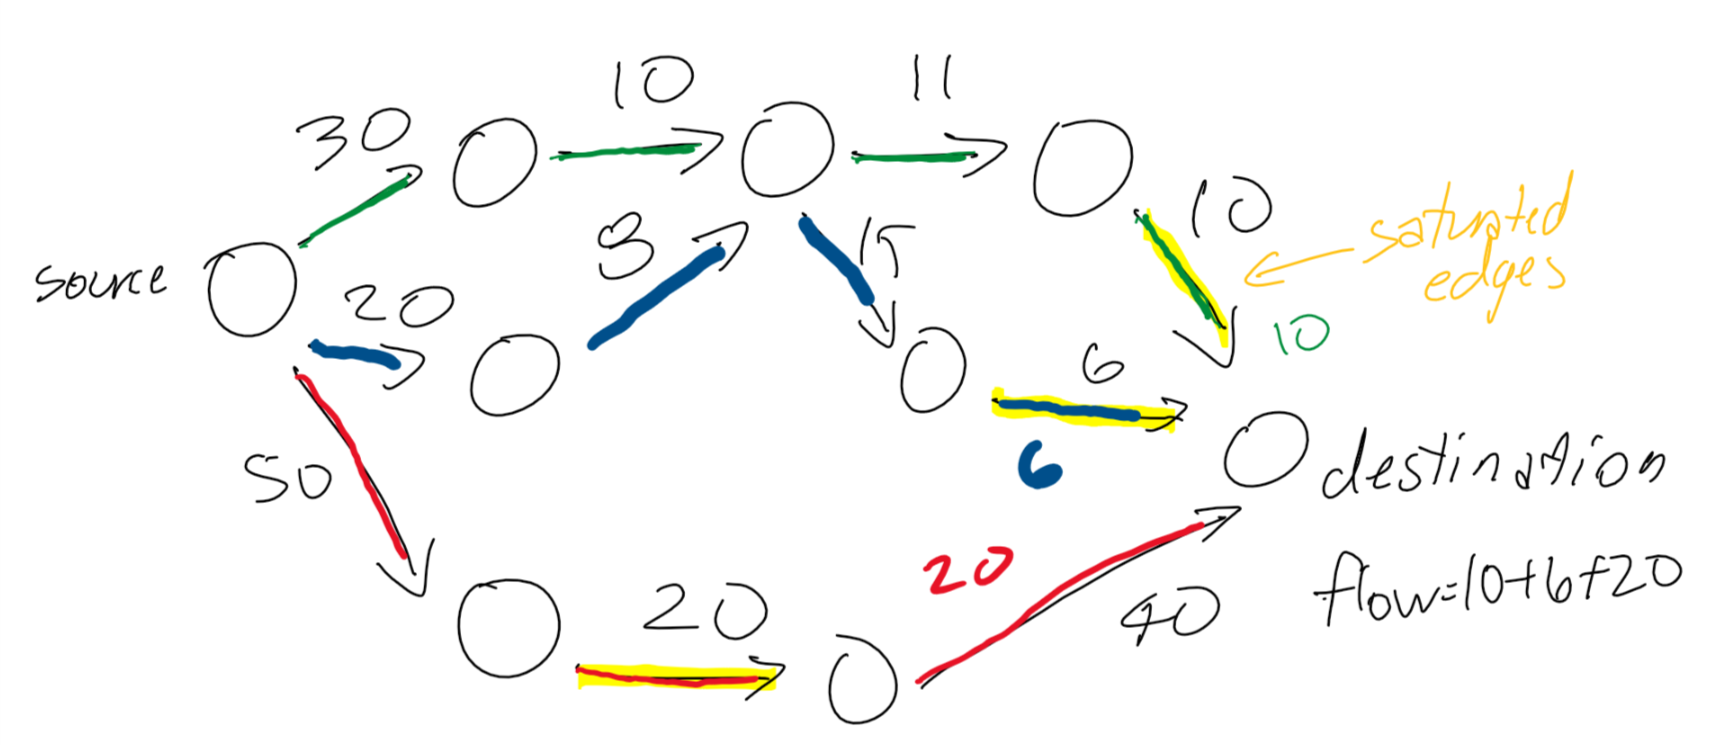
\includegraphics[width=3in]{network_flow.png}
  \caption{Network flow from a source to a destination along edges with capacity}
  \label{fig:network_flow}
\end{figure}

In this example, we see that the edges with capacity 10, 6, and 20 become saturated and constraint the flow from the source to the destination. It turns out that these edges form a min s-t cut according to the min max theorem. In a flow network, a s-t cut is a set of edges that when removed isolates the source and destination. The min s-t cut has a minimum value of weight associated with the set of edges. So if we find the min s-t cut, the weight of the edges is equal to the max flow from the source to the destination.

\newpage
\subsubsection{ Min-Max Theorem}
The max-flow min-cut theorem states that in a flow network, the amount of maximum flow is equal to capacity of the minimum cut.

It turns out that matching problems can be modeled as a max flow problem by adding dummy source and destination nodes, and edges with  capacity 1 from the source to the girls and from the boys to the destination, and of infinite capacity between boys and girls.

\begin{figure}[!ht]
  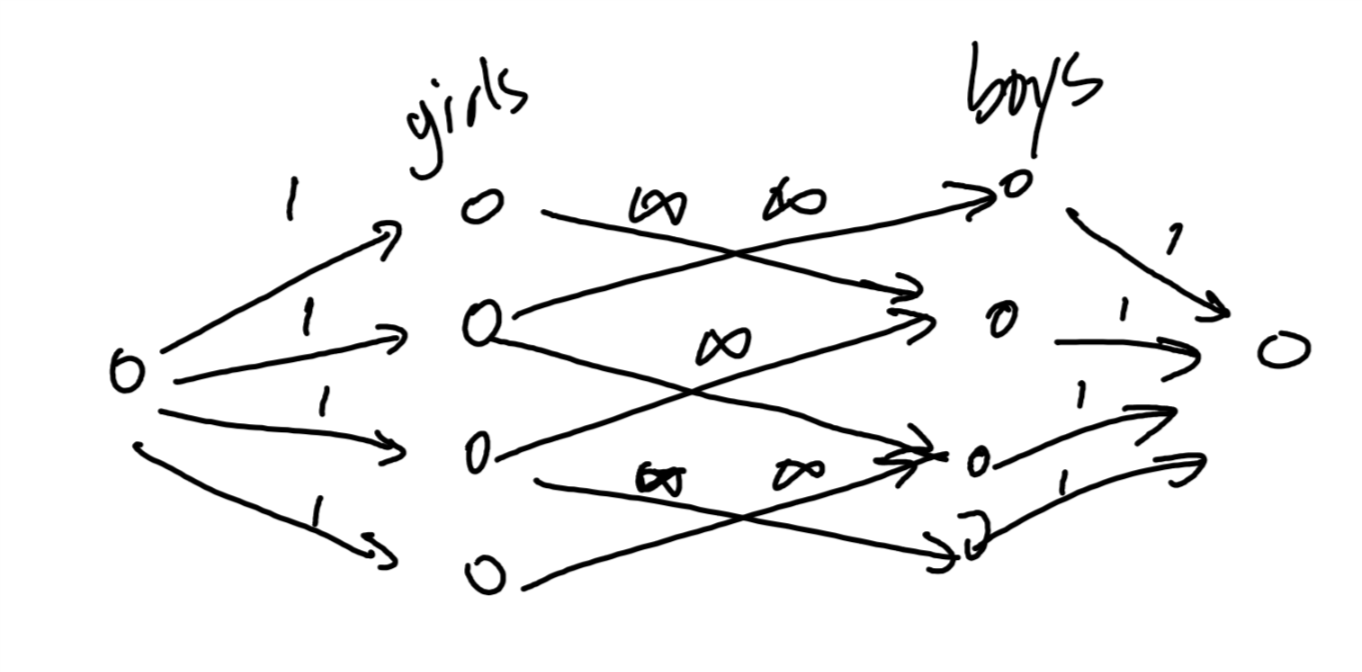
\includegraphics[width=3in]{matching_flow.png}
  \caption{Matching Problem as a network flow}
  \label{fig:matching_flow}
\end{figure}

\section{Appendix}
In this section, we'll write the primal using vectors and arrays. Note that this was not covered in lecture, and is here just for extra information

We can rewrite the objective function as 
\newline $\textbf{c}'\textbf{x}$
\newline where $\textbf{x}$ is the vector of decision variables and $\textbf{c}$ is the vector of coefficients in the objective function.
\newline Bold face indicates vectors, and $\textbf{a}'\textbf{b}$ is the transpose of $\textbf{a}$ times $\textbf{b}$.
\newline Then the coefficients of the constraints form the matrix
$$
A=
\begin{bmatrix} 
a_{11} & a_{12} & \ldots & a_{1n} \\ 
a_{21} & a_{22} & \ldots & a_{2n}\\
\vdots\\
a_{m1} & a_{m2} & \ldots & a_{mn}
\end{bmatrix}
$$
with rows $\textbf{a}_i$ and columns $\textbf{A}_j$
\newline So the primal can be rewritten into the following structure
\newline minimize 
\newline $\textbf{c}'\textbf{x}$
\newline subject to 
\newline $\textbf{a}_i'\textbf{x} \geq b_i \in M_1 $
\newline $\textbf{a}_i'\textbf{x} \leq b_i, i \in M_2,$
\newline $\textbf{a}_i'\textbf{x} = b_i, i \in M_3,$
\newline $x_j \geq 0, j \in N_1$
\newline $x_j \leq 0, j \in N_2$
\newline $x_j$ free, $j \in N_3$

\newpage
The dual then has the structure 
\newline maximize 
\newline $\textbf{p}'\textbf{b}$
\newline subject to 
\newline $p_i \geq 0, i \in M_1$
\newline $p_i \leq 0, i \in M_2$
\newline $p_i$ free, $i \in M_3$
\newline $\textbf{p}'\textbf{A}_j \leq c_j, j \in N_1 $
\newline $\textbf{p}'\textbf{A}_j \geq c_j, j \in M_2,$
\newline $\textbf{p}'\textbf{A}_j = c_j, j \in N_3,$



\end{document}





